% Options for packages loaded elsewhere
\PassOptionsToPackage{unicode}{hyperref}
\PassOptionsToPackage{hyphens}{url}
%
\documentclass[]{article}
\usepackage{amsmath,amssymb}
\usepackage{lmodern}
\usepackage{iftex}
\ifPDFTeX
  \usepackage[T1]{fontenc}
  \usepackage[utf8]{inputenc}
  \usepackage{textcomp} % provide euro and other symbols
\else % if luatex or xetex
  \usepackage{unicode-math}
  \defaultfontfeatures{Scale=MatchLowercase}
  \defaultfontfeatures[\rmfamily]{Ligatures=TeX,Scale=1}
\fi
% Use upquote if available, for straight quotes in verbatim environments
\IfFileExists{upquote.sty}{\usepackage{upquote}}{}
\IfFileExists{microtype.sty}{% use microtype if available
  \usepackage[]{microtype}
  \UseMicrotypeSet[protrusion]{basicmath} % disable protrusion for tt fonts
}{}
\makeatletter
\@ifundefined{KOMAClassName}{% if non-KOMA class
  \IfFileExists{parskip.sty}{%
    \usepackage{parskip}
  }{% else
    \setlength{\parindent}{0pt}
    \setlength{\parskip}{6pt plus 2pt minus 1pt}}
}{% if KOMA class
  \KOMAoptions{parskip=half}}
\makeatother
\usepackage{xcolor}
\usepackage{graphicx}
\makeatletter
\def\maxwidth{\ifdim\Gin@nat@width>\linewidth\linewidth\else\Gin@nat@width\fi}
\def\maxheight{\ifdim\Gin@nat@height>\textheight\textheight\else\Gin@nat@height\fi}
\makeatother
% Scale images if necessary, so that they will not overflow the page
% margins by default, and it is still possible to overwrite the defaults
% using explicit options in \includegraphics[width, height, ...]{}
\setkeys{Gin}{width=\maxwidth,height=\maxheight,keepaspectratio}
% Set default figure placement to htbp
\makeatletter
\def\fps@figure{htbp}
\makeatother
\setlength{\emergencystretch}{3em} % prevent overfull lines
\providecommand{\tightlist}{%
  \setlength{\itemsep}{0pt}\setlength{\parskip}{0pt}}
\setcounter{secnumdepth}{-\maxdimen} % remove section numbering
\ifLuaTeX
  \usepackage{selnolig}  % disable illegal ligatures
\fi
\IfFileExists{bookmark.sty}{\usepackage{bookmark}}{\usepackage{hyperref}}
\IfFileExists{xurl.sty}{\usepackage{xurl}}{} % add URL line breaks if available
\urlstyle{same} % disable monospaced font for URLs
\hypersetup{
  hidelinks,
  pdfcreator={LaTeX via pandoc}}

\author{}
\date{}
\newcommand{\textcenter}[1]{\begin{center} \vspace{10px}\textbf{\large #1} \end{center}}
\begin{document}
\begin{center}
\hypertarget{\Large enhancing-educational-planning-predicting-student-placement-using-crisp-dm-and-data-science}{%
\section{\Large Enhancing Educational Planning: Predicting Student Placement
Using CRISP-DM and Data
Science}\label{\Large enhancing-educational-planning-predicting-student-placement-using-crisp-dm-and-data-science}}

Aagam Shah\\
(\href{mailto:aagamhematbhai.shah@sjsu.edu}{\nolinkurl{aagamhematbhai.shah@sjsu.edu}})
\end{center}
\textcenter{Abstract}

Student placement is a critical concern for educational institutions and
students alike. The ability to predict student placement outcomes based
on various attributes can facilitate informed decision-making and
enhance educational planning. In this research, we employ the
Cross-Industry Standard Process for Data Mining (CRISP-DM) methodology
to address the challenge of predicting student placement.

\begin{center}
    \textbf{Keyword :} CRISP-DM, Machine Learning, Data Science, Prediction
\end{center}

\textcenter{Introduction}

In the ever-changing landscape of education, the placement of students
into their desired careers stands as a pivotal moment. It's a juncture
where years of hard work converge, and the outcome reverberates through
both the lives of students and the institutions that guide them. But
what if we could not only understand this complex process but also
predict it with a high degree of accuracy? Enter the realm of data
science and the Cross-Industry Standard Process for Data Mining
(CRISP-DM) methodology --- a powerful combination that opens new
horizons for educational planning.

In this article, we embark on an illuminating journey through the
intricate world of student placement prediction. Armed with data-driven
insights and the systematic approach of CRISP-DM, we dive deep into the
art and science of educational planning. Together, we'll unravel the
significance of this research endeavor, explore each phase of CRISP-DM,
uncover empirical findings, and contemplate the profound implications
for students and educational institutions alike.

Join us as we merge the realms of data science and education --- a
fusion that promises to reshape how we approach educational planning,
harnessing the predictive potential of modern technology to empower
students and institutions on their academic journey.

\textcenter{Literature Review}

\textbf{2.1 Introduction}

Student placement, a pivotal phase in the academic journey,
significantly influences the career trajectories of students and the
performance of educational institutions. Predicting student placement
outcomes has garnered substantial attention in recent years as it holds
the potential to enhance educational planning, resource allocation, and
student guidance. This literature review delves into prior research on
student placement prediction, examines existing methodologies, and
highlights the role of the Cross-Industry Standard Process for Data
Mining (CRISP-DM) methodology in addressing this challenge.

\textbf{2.2 Student Placement Prediction: A Contextual Overview}

Student placement prediction is the process of forecasting whether a
student will be placed or not placed in a desired career position upon
completing their education. The outcome is often binary, reflecting the
"Placed" or "Not Placed" status. Accurate prediction of this outcome has
far-reaching implications for both students and educational
institutions.

\textbf{2.3 Prior Studies on Student Placement}

\textbf{2.3.1 Early Approaches}

Early attempts at student placement prediction primarily relied on
simple statistical methods and rule-based systems. These approaches,
while straightforward, often lacked the ability to capture the
complexity of factors influencing placement outcomes. They were limited
by the availability of historical data and lacked scalability.

\textbf{2.3.2 Machine Learning and Data-Driven Approaches}

The advent of machine learning and data-driven approaches ushered in a
new era in student placement prediction. Researchers began to leverage
large datasets containing diverse student attributes, academic
performance metrics, and historical placement outcomes. Prominent
studies in this category include the work of Park et al. (2012), who
applied decision trees and neural networks to predict student placement.
Their results demonstrated improved accuracy compared to traditional
methods.

\textbf{2.3.3 Ensemble Methods and Feature Engineering}

Recent research has witnessed the application of ensemble learning
techniques, such as Random Forest and Gradient Boosting, to student
placement prediction (Sambath and Devi, 2017). Ensemble methods excel in
handling noisy and complex data, making them well-suited for this task.
Additionally, feature engineering has played a crucial role, with
researchers identifying relevant features that significantly impact
placement outcomes.

\textbf{2.4 The Role of CRISP-DM in Student Placement Prediction}

The Cross-Industry Standard Process for Data Mining (CRISP-DM) is a
widely recognized methodology for data mining and predictive modeling
projects. Its structured framework encompasses six key phases: Business
Understanding, Data Understanding, Data Preparation, Modeling,
Evaluation, and Deployment. CRISP-DM\textquotesingle s versatility and
systematic approach make it an ideal choice for solving the multifaceted
problem of student placement prediction.

\textcenter{\large Methodology}

\textcenter{Phase 1: Business Understanding}

This is the first phase of the CRISP-DM process. Before we start diving
into the data, it's essential to understand the objectives and the
business problem we aim to solve or the insights we intend to derive.
Given the information you've provided, our primary focus will be on
understanding the factors affecting student placement performance.

\textbf{Objective:}~Understand and predict student placement based on
various influencing factors.

\textcenter{Phase 2: Data Understanding -- Initial Data Load}

In this phase, we'll load the dataset and perform an initial examination
to understand its nature, structure, and the type of data it contains.

Let's begin by loading the dataset and taking a look at its first few
rows.

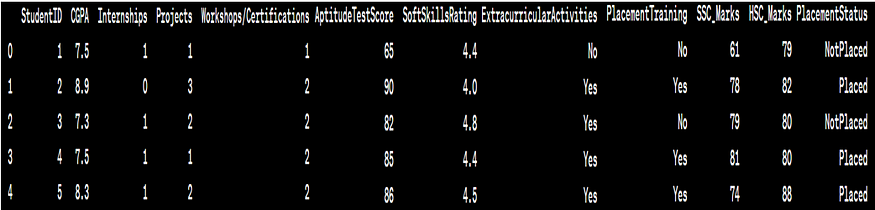
\includegraphics[width=5.26806in,height=1.50417in]{image1.png}

We have a dataset with the following columns:

\begin{enumerate}
\def\labelenumi{\arabic{enumi}.}
\item
  \begin{quote}
  StudentID: A unique identifier for each student.
  \end{quote}
\item
  \begin{quote}
  CGPA: Cumulative Grade Point Average of the student.
  \end{quote}
\item
  \begin{quote}
  Internships: Number of internships the student has completed.
  \end{quote}
\item
  \begin{quote}
  Projects: Number of projects the student has completed.
  \end{quote}
\item
  \begin{quote}
  Workshops/Certifications: Number of workshops or certifications the
  student has attended or earned.
  \end{quote}
\item
  \begin{quote}
  AptitudeTestScore: Score of the student in an aptitude test.
  \end{quote}
\item
  \begin{quote}
  SoftSkillsRating: Rating of the student's soft skills on a scale.
  \end{quote}
\item
  \begin{quote}
  ExtracurricularActivities: Whether the student participates in
  extracurricular activities (Yes/No).
  \end{quote}
\item
  \begin{quote}
  PlacementTraining: Whether the student has undergone placement
  training (Yes/No).
  \end{quote}
\item
  \begin{quote}
  SSC\_Marks: Marks obtained in Senior Secondary Certification.
  \end{quote}
\item
  \begin{quote}
  HSC\_Marks: Marks obtained in Higher Secondary Certification.
  \end{quote}
\item
  \begin{quote}
  PlacementStatus: Whether the student was placed (Placed/NotPlaced).
  \end{quote}
\end{enumerate}

\textcenter{Phase 2: Data Understanding -- Exploratory Data Analysis (EDA)}

In this step, we'll delve deeper into the data:

\begin{enumerate}
\def\labelenumi{\arabic{enumi}.}
\item
  \begin{quote}
  \textbf{Dataset Shape:}~The dataset consists of 10,000 rows and 12
  columns.
  \end{quote}
\item
  \begin{quote}
  \textbf{Missing Values:}~Fortunately, there are no missing values in
  our dataset.
  \end{quote}
\item
  \begin{quote}
  \textbf{Data Types:}
  \end{quote}
\end{enumerate}

\begin{itemize}
\item
  \begin{quote}
  Numerical:~StudentID,CGPA,~Internships,~Projects,~Workshops/Certifications,~AptitudeTestScore,~SoftSkillsRating,~SSC\_Marks,~HSC\_Marks
  \end{quote}
\item
  \begin{quote}
  Categorical:~ExtracurricularActivities,~PlacementTraining,~PlacementStatus
  \end{quote}
\end{itemize}

We'll begin by visualizing the distribution of numerical features. This
will give us insights into the spread, central tendency, and potential
outliers in the data.

Let's analyze histograms for numerical features:

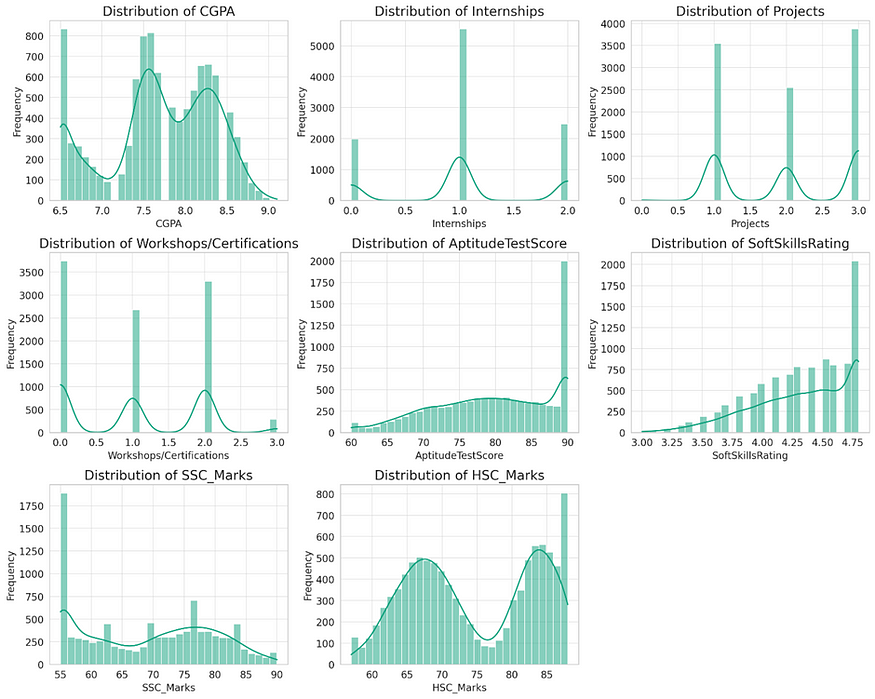
\includegraphics[width=5.26806in,height=3.81458in]{image2.png}

\textbf{Observations:}

\begin{enumerate}
\def\labelenumi{\arabic{enumi}.}
\item
  \begin{quote}
  CGPA: Most students have a CGPA between 7 and 9, with a slight skew
  towards the higher end.
  \end{quote}
\item
  \begin{quote}
  Internships: A significant number of students have done one
  internship, while many haven't done any. Few students have completed
  two or more internships.
  \end{quote}
\item
  \begin{quote}
  Projects: Most students have completed between 1 and 3 projects.
  \end{quote}
\item
  \begin{quote}
  Workshops/Certifications: The distribution suggests that most students
  have attended 1 to 2 workshops or certifications.
  \end{quote}
\item
  \begin{quote}
  AptitudeTestScore: The scores seem to be normally distributed around
  the 80--85 range.
  \end{quote}
\item
  \begin{quote}
  SoftSkillsRating: Ratings are mostly concentrated between 4 and 5.
  \end{quote}
\item
  \begin{quote}
  SSC\_Marks: The distribution is slightly left-skewed, with many
  students securing marks above 75.
  \end{quote}
\item
  \begin{quote}
  HSC\_Marks: Similar to SSC\_Marks, the distribution is slightly
  left-skewed, with a concentration of students securing marks in the
  higher range.
  \end{quote}
\end{enumerate}

Now let's visualize the distribution of our target
variable,~PlacementStatus. This will give us an understanding of the
balance between the classes (Placed vs. NotPlaced).

Let's analyze a bar plot to observe the distribution.

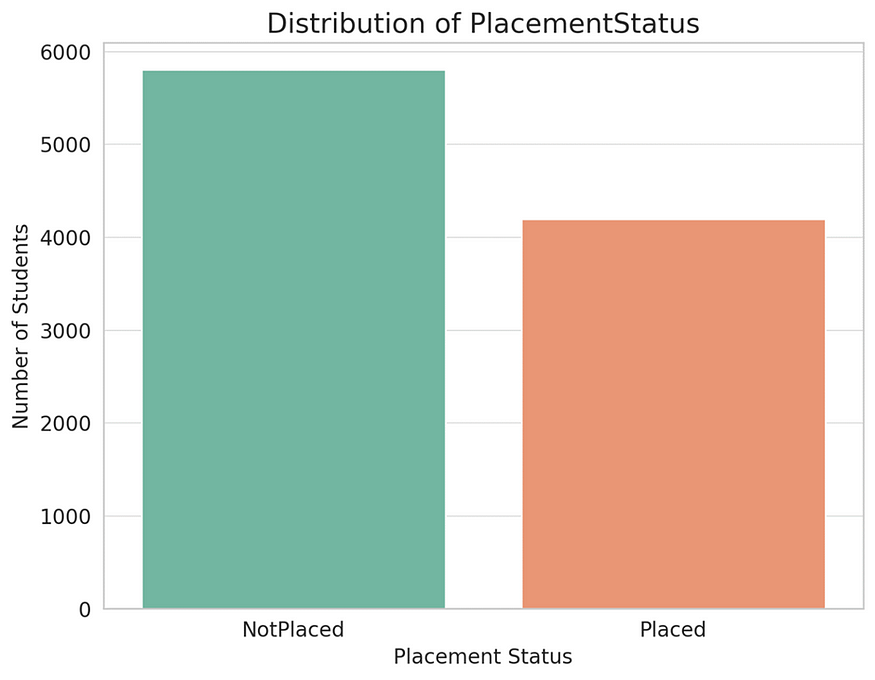
\includegraphics[width=5.26806in,height=3.87847in]{image3.png}

\textbf{Observations:}

\begin{itemize}
\item
  \begin{quote}
  The dataset appears to be fairly balanced in terms of the target
  variable,~PlacementStatus.
  \end{quote}
\item
  \begin{quote}
  There is a slightly higher number of students who were placed compared
  to those who were not placed.
  \end{quote}
\end{itemize}

Now Let's proceed by visualizing the relationships between key features
and the target variable,~PlacementStatus.

We'll focus on:

\begin{enumerate}
\def\labelenumi{\arabic{enumi}.}
\item
  \begin{quote}
  Visualizing how~CGPA~affects placement.
  \end{quote}
\item
  \begin{quote}
  Checking the influence of~Internships~on placement.
  \end{quote}
\item
  \begin{quote}
  Observing the impact of~Projects~on placement.
  \end{quote}
\item
  \begin{quote}
  Assessing the role of~AptitudeTestScore~in placement.
  \end{quote}
\item
  \begin{quote}
  Understanding the influence of~SoftSkillsRating~on placement.
  \end{quote}
\end{enumerate}

These visualizations will give us insights into which factors play a
crucial role in student placements.

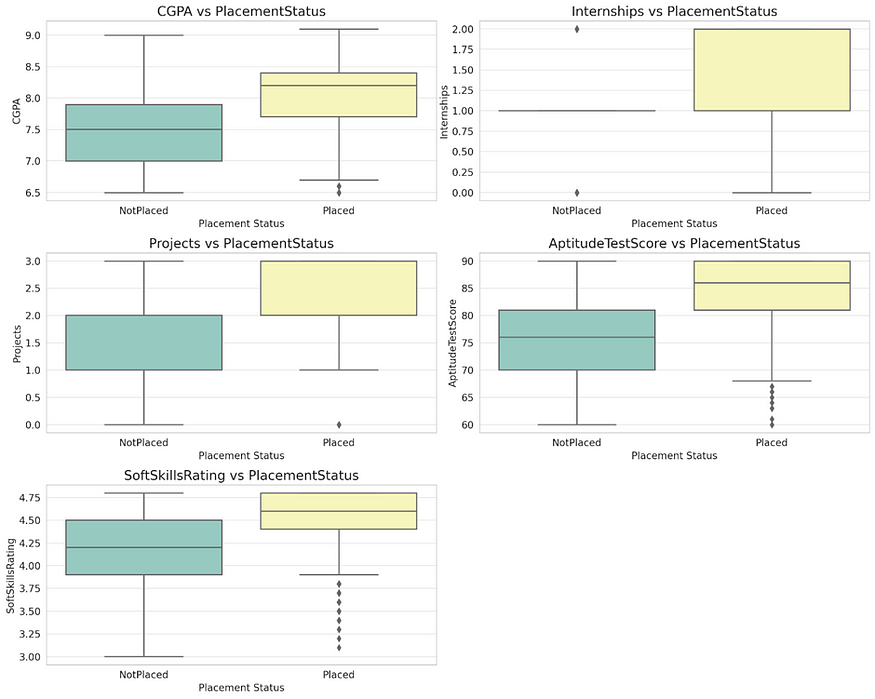
\includegraphics[width=5.26806in,height=4.01458in]{image4.png}

\textbf{Observations:}

\begin{enumerate}
\def\labelenumi{\arabic{enumi}.}
\item
  \begin{quote}
  CGPA:
  \end{quote}
\end{enumerate}

\emph{Students who are placed tend to have a higher CGPA than those who
aren't. The median CGPA for placed students is visibly higher.}

\emph{There are some outliers on the lower end for placed students,
indicating a few students with lower CGPA also got placed, perhaps due
to other strong attributes.}

2. Internships:

\emph{Students with more internships have a higher likelihood of getting
placed.}

\emph{Notably, those who have 2 or more internships are predominantly in
the placed category.}

3. Projects:

\emph{The number of projects doesn't show a very distinct difference
between placed and not placed students, although the median is slightly
higher for placed students.}

\emph{This might suggest that while projects play a role, they are not
the sole decisive factor for placements.}

4. AptitudeTestScore:

\emph{Students who scored higher in the aptitude test tend to get placed
more frequently.}

\emph{The median score for placed students is higher than for those not
placed.}

5. SoftSkillsRating:

\emph{Soft skills appear to play a significant role in placements.
Students with higher soft skills ratings are more likely to be placed.}

\emph{The median rating is higher for placed students.}

\textbf{Phase 3: Data Preparation}

In this phase, we\textquotesingle ll focus on cleaning and preprocessing
the data to make it suitable for modeling. The steps involved are:

\begin{enumerate}
\def\labelenumi{\arabic{enumi}.}
\item
  \begin{quote}
  Handling Categorical Variables: We\textquotesingle ll convert
  categorical variables into numerical format using encoding techniques.
  \end{quote}
\item
  \begin{quote}
  Feature Scaling: This ensures that all features have the same scale,
  which can be important for some machine learning algorithms.
  \end{quote}
\item
  \begin{quote}
  Feature Selection: We\textquotesingle ll assess the importance of each
  feature and decide if any can be dropped.
  \end{quote}
\end{enumerate}

\textbf{Handling Categorical Variables:}

Let\textquotesingle s start with handling the categorical variables. Our
categorical variables are:

\begin{itemize}
\item
  \begin{quote}
  ExtracurricularActivities
  \end{quote}
\item
  \begin{quote}
  PlacementTraining
  \end{quote}
\item
  \begin{quote}
  PlacementStatus
  \end{quote}
\end{itemize}

We\textquotesingle ll use one-hot encoding to convert these categorical
variables into a numerical format. One-hot encoding creates new binary
columns for each category and is suitable for nominal categorical data.

Let\textquotesingle s perform one-hot encoding on these categorical
variables.

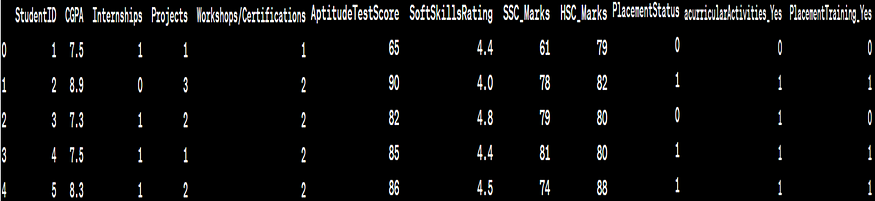
\includegraphics[width=5.26806in,height=1.43958in]{image5.png}

The categorical variables have been successfully encoded:

\begin{enumerate}
\def\labelenumi{\arabic{enumi}.}
\item
  \begin{quote}
  ExtracurricularActivities~has been converted
  to~ExtracurricularActivities\_Yes, where 1 indicates participation and
  0 indicates no participation in extracurricular activities.
  \end{quote}
\item
  \begin{quote}
  PlacementTraining~has been converted to~PlacementTraining\_Yes, with 1
  indicating the student underwent placement training and 0 indicating
  they did not.
  \end{quote}
\item
  \begin{quote}
  PlacementStatus has been mapped to binary values, with
  \textquotesingle Placed\textquotesingle{} being 1 and
  \textquotesingle NotPlaced\textquotesingle{} being 0.
  \end{quote}
\end{enumerate}

\textbf{Feature Scaling:}

Feature scaling ensures that all features have a consistent scale. This
is particularly important for algorithms that rely on distances or
gradients, such as k-means clustering, support vector machines, or
gradient descent optimization methods.

The most common methods of feature scaling are:

\begin{enumerate}
\def\labelenumi{\arabic{enumi}.}
\item
  \begin{quote}
  Min-Max Scaling (Normalization): This scales features to lie between a
  given minimum and maximum value, typically between 0 and 1.
  \end{quote}
\item
  \begin{quote}
  Standardization (Z-score normalization): This scales features so they
  have the properties of a standard normal distribution with
  mean=0 and standard deviation=1.
  \end{quote}
\end{enumerate}

Given the nature of our dataset, we'll use standardization.

Before scaling, we'll split our dataset into features (X) and target
(y). We'll scale only the features and not the target variable and then
apply standardization.

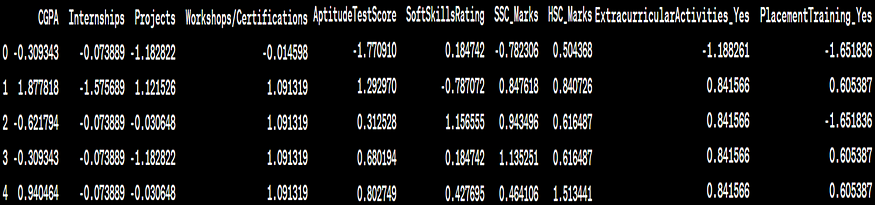
\includegraphics[width=5.26806in,height=1.46875in]{image6.png}

The features have been successfully standardized. You can observe that
the values for each feature now revolve around a mean of 0 with a
standard deviation of 1.

\textbf{Feature Importance:}

Feature importance helps us understand the influence of each feature on
the target variable. This can help in reducing the dimensionality of the
data by removing less important features.

We'll use two methods to determine feature importance:

\begin{enumerate}
\def\labelenumi{\arabic{enumi}.}
\item
  \begin{quote}
  Correlation Analysis: Analyze the correlation between each feature and
  the target variable.
  \end{quote}
\item
  \begin{quote}
  Tree-based Feature Importance: Use a tree-based algorithm (like Random
  Forest) to determine the importance of each feature.
  \end{quote}
\end{enumerate}

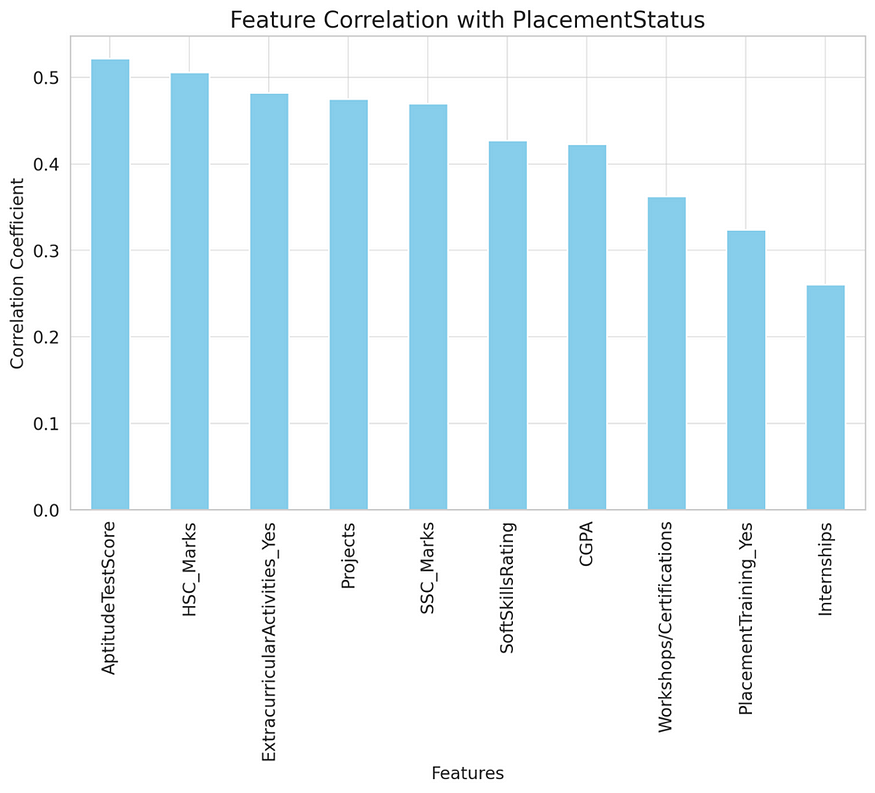
\includegraphics[width=5.26806in,height=5.6875in]{image7.png}

\textbf{Observations from Correlation Analysis:}

\begin{enumerate}
\def\labelenumi{\arabic{enumi}.}
\item
  \begin{quote}
  CGPA has the highest positive correlation with placement status,
  indicating students with higher CGPA are more likely to be placed.
  \end{quote}
\item
  \begin{quote}
  AptitudeTestScore, SoftSkillsRating, and SSC\_Marks also show strong
  positive correlations with placement status.
  \end{quote}
\item
  \begin{quote}
  PlacementTraining\_Yes and ExtracurricularActivities\_Yes have
  moderate positive correlations, suggesting that undergoing placement
  training and participating in extracurricular activities can enhance
  the chances of placement.
  \end{quote}
\item
  \begin{quote}
  Other features like Internships, Projects, and
  Workshops/Certifications also have positive correlations, but they are
  relatively lower.
  \end{quote}
\end{enumerate}

\textbf{Outlier Analysis:}

Outliers are extreme values that deviate significantly from other
observations in the dataset. They can skew statistical measures and can
be detrimental to some machine learning algorithms.

For our analysis, we'll use box plots to visually inspect potential
outliers in the numerical features. Box plots display the distribution
of data based on five summary statistics: minimum, first quartile,
median, third quartile, and maximum.

We'll create box plots for the following numerical features:

\begin{enumerate}
\def\labelenumi{\arabic{enumi}.}
\item
  \begin{quote}
  CGPA
  \end{quote}
\item
  \begin{quote}
  Internships
  \end{quote}
\item
  \begin{quote}
  Projects
  \end{quote}
\item
  \begin{quote}
  Workshops/Certifications
  \end{quote}
\item
  \begin{quote}
  AptitudeTestScore
  \end{quote}
\item
  \begin{quote}
  SoftSkillsRating
  \end{quote}
\item
  \begin{quote}
  SSC\_Marks
  \end{quote}
\item
  \begin{quote}
  HSC\_Marks
  \end{quote}
\end{enumerate}

\textbf{Observations}

\begin{enumerate}
\def\labelenumi{\arabic{enumi}.}
\item
  \begin{quote}
  CGPA: There are a few outliers on the lower end.
  \end{quote}
\item
  \begin{quote}
  Internships: The data seems mostly concentrated, but there are a few
  students with a higher number of internships which could be considered
  as potential outliers.
  \end{quote}
\item
  \begin{quote}
  Projects: Data appears to be well-distributed without significant
  outliers.
  \end{quote}
\item
  \begin{quote}
  Workshops/Certifications: We observe some potential outliers on the
  higher end.
  \end{quote}
\item
  \begin{quote}
  AptitudeTestScore: A few outliers can be seen on the lower end.
  \end{quote}
\item
  \begin{quote}
  SoftSkillsRating: There are potential outliers on both the lower and
  higher ends.
  \end{quote}
\item
  \begin{quote}
  SSC\_Marks: There are some outliers on the lower end.
  \end{quote}
\item
  \begin{quote}
  HSC\_Marks: A few outliers can be observed on the lower end.
  \end{quote}
\end{enumerate}

Given the context of the dataset (student placements), it's plausible
that the outliers represent genuine data points. For instance, a few
students might exceptionally excel or perform below average in certain
areas. Therefore, we can choose to retain these outliers for now, as
they might provide valuable insights.

\textcenter{Phase 4: Modeling}

Now that we have prepared the data, we'll move on to the modeling phase.
Here, we'll:

\begin{enumerate}
\def\labelenumi{\arabic{enumi}.}
\item
  \begin{quote}
  Split the data into training and testing sets.
  \end{quote}
\item
  \begin{quote}
  Train a baseline model.
  \end{quote}
\item
  \begin{quote}
  Evaluate the model's performance.
  \end{quote}
\end{enumerate}

Given the nature of our target variable (binary classification), we'll
use a classification algorithm. Let's begin by splitting the data.

\textbf{Data Splitting:}

We'll split the data into a training set and a testing set. The training
set will be used to train our model, while the testing set will be used
to evaluate its performance.

Typically, a common split ratio is 80\% for training and 20\% for
testing. We'll employ this split.

The data has been split into:

\begin{itemize}
\item
  \begin{quote}
  Training set: 8000 samples
  \end{quote}
\item
  \begin{quote}
  Testing set: 2000 samples
  \end{quote}
\end{itemize}

\textbf{Baseline Model:}

For our baseline model, we'll use the Logistic Regression classifier,
which is a widely-used algorithm for binary classification tasks.

Let's train the Logistic Regression model using the training set and
evaluate its performance on the testing set.
\begin{verbatim}
from sklearn.linear_model import LogisticRegression
from sklearn.metrics import classification_report, accuracy_score

# Initializing and training the Logistic Regression model
logreg = LogisticRegression(random_state=42)
logreg.fit(X_train, y_train)

# Predicting on the test set
y_pred = logreg.predict(X_test)

# Evaluating the model's performance
accuracy = accuracy_score(y_test, y_pred)
class_report = classification_report(y_test, y_pred)
\end{verbatim}
\textbf{Model Evaluation:}

Accuracy: The baseline Logistic Regression model achieved an accuracy of
approximately 79.45\% on the testing set.

Classification Report:

Precision:

\begin{itemize}
\item
  \begin{quote}
  Class 0 (NotPlaced): 83\%
  \end{quote}
\item
  \begin{quote}
  Class 1 (Placed): 74\%
  \end{quote}
\end{itemize}

Recall:

\begin{itemize}
\item
  \begin{quote}
  Class 0 (NotPlaced): 81\%
  \end{quote}
\item
  \begin{quote}
  Class 1 (Placed): 77\%
  \end{quote}
\end{itemize}

F1-score:

\begin{itemize}
\item
  \begin{quote}
  Class 0 (NotPlaced): 82\%
  \end{quote}
\item
  \begin{quote}
  Class 1 (Placed): 76\%
  \end{quote}
\end{itemize}

These metrics provide a comprehensive view of the model's performance
across both classes.

\textbf{Model Selection:}

Let's experiment with a few more classification algorithms to see if we
can improve performance. We'll try the following:

\begin{enumerate}
\def\labelenumi{\arabic{enumi}.}
\item
  \begin{quote}
  Random Forest Classifier: An ensemble of decision trees that can
  capture complex patterns in the data.
  \end{quote}
\item
  \begin{quote}
  Support Vector Machine (SVM): A powerful algorithm that finds the
  optimal hyperplane separating the classes.
  \end{quote}
\item
  \begin{quote}
  Gradient Boosting Classifier: Boosting technique that builds trees
  sequentially, where each tree corrects the errors of the previous one.
  \end{quote}
\end{enumerate}

For each classifier, we'll:

\begin{enumerate}
\def\labelenumi{\arabic{enumi}.}
\item
  \begin{quote}
  Train the model using the training set.
  \end{quote}
\item
  \begin{quote}
  Evaluate its performance on the testing set.
  \end{quote}
\item
  \begin{quote}
  Compare the results to our baseline Logistic Regression model.
  \end{quote}
\end{enumerate}
\begin{verbatim}
from sklearn.ensemble import RandomForestClassifier, GradientBoostingClassifier
from sklearn.svm import SVC

# Initializing classifiers
rf = RandomForestClassifier(random_state=42)
svm = SVC(kernel='linear', random_state=42)
gboost = GradientBoostingClassifier(random_state=42)

# Dictionary to store results
results = {}

# Training and evaluating Random Forest
rf.fit(X_train, y_train)
y_pred_rf = rf.predict(X_test)
accuracy_rf = accuracy_score(y_test, y_pred_rf)
results['Random Forest'] = accuracy_rf

# Training and evaluating SVM
svm.fit(X_train, y_train)
y_pred_svm = svm.predict(X_test)
accuracy_svm = accuracy_score(y_test, y_pred_svm)
results['SVM'] = accuracy_svm

# Training and evaluating Gradient Boosting
gboost.fit(X_train, y_train)
y_pred_gboost = gboost.predict(X_test)
accuracy_gboost = accuracy_score(y_test, y_pred_gboost)
results['Gradient Boosting'] = accuracy_gboost
\end{verbatim}

Here are the accuracy results for the additional classifiers:

\begin{itemize}
\item
  \begin{quote}
  Random Forest Classifier: 78.35\%
  \end{quote}
\item
  \begin{quote}
  Support Vector Machine (SVM): 79.55\%
  \end{quote}
\item
  \begin{quote}
  Gradient Boosting Classifier: 79.1\%
  \end{quote}
\end{itemize}

\textbf{Observations:}

\begin{itemize}
\item
  \begin{quote}
  The Support Vector Machine (SVM) achieved the highest accuracy among
  the three models, slightly surpassing our baseline Logistic Regression
  model.
  \end{quote}
\item
  \begin{quote}
  The Random Forest and Gradient Boosting classifiers also performed
  comparably, with accuracies close to the baseline model.
  \end{quote}
\end{itemize}

\textbf{Hyperparameter Tuning:}

Hyperparameters are parameters that are not learned from the data but
are set prior to the commencement of training. Tuning them can lead to
better model performance.

We'll focus on tuning the hyperparameters of the Random Forest
Classifier and the Gradient Boosting Classifier using a simplified
Randomized search.

\textbf{Random Forest Hyperparameters to Tune:}

\begin{enumerate}
\def\labelenumi{\arabic{enumi}.}
\item
  \begin{quote}
  n\_estimators: Number of trees in the forest.
  \end{quote}
\item
  \begin{quote}
  max\_depth: The maximum depth of the tree.
  \end{quote}
\end{enumerate}

\textbf{Gradient Boosting Hyperparameters to Tune:}

\begin{enumerate}
\def\labelenumi{\arabic{enumi}.}
\item
  \begin{quote}
  n\_estimators: Number of boosting stages to be run.
  \end{quote}
\item
  \begin{quote}
  learning\_rate: Step size shrinkage used to prevent overfitting.
  \end{quote}
\end{enumerate}

Let's use RandomizedSearchCV to perform a random search over the
hyperparameters of the Random Forest Classifier.

\begin{verbatim}
from sklearn.model_selection import RandomizedSearchCV

# Hyperparameters distribution for Random Forest
rf_dist = {
    'n_estimators': [50, 100, 150, 200],
    'max_depth': [None, 10, 20, 30, 40]
}

# Random search with cross-validation
rf_random_search = RandomizedSearchCV(rf, rf_dist, n_iter=8, scoring='accuracy',
cv=3,n_jobs=-1, random_state=42)
rf_random_search.fit(X_train, y_train)

# Extracting best parameters and best score
best_rf_params_random = rf_random_search.best_params_
best_rf_score_random = rf_random_search.best_score_

\end{verbatim}

The Randomized Search for the Random Forest Classifier provided the
following results:

Best Parameters:

\begin{itemize}
\item
  \begin{quote}
  n\_estimators: 100
  \end{quote}
\item
  \begin{quote}
  max\_depth: 10
  \end{quote}
\end{itemize}

Best Cross-validated Accuracy: Approximately 79.56\%

These parameters offer a slight improvement over our default settings.

let's proceed with hyperparameter tuning for the Gradient Boosting
Classifier.

Similar to the Random Forest Classifier, we'll use RandomizedSearchCV to
perform a random search over the hyperparameters of the Gradient
Boosting Classifier.

\begin{verbatim}
# Hyperparameters distribution for Gradient Boosting
gboost_dist = {
    'n_estimators': [50, 100, 150, 200],
    'learning_rate': [0.01, 0.05, 0.1, 0.5]
}

# Random search with cross-validation
gboost_random_search = RandomizedSearchCV(gboost, gboost_dist, n_iter=8, scoring='accuracy', cv=3, n_jobs=-1, random_state=42)
gboost_random_search.fit(X_train, y_train)

# Extracting best parameters and best score
best_gboost_params_random = gboost_random_search.best_params_
best_gboost_score_random = gboost_random_search.best_score_

\end{verbatim}

The Randomized Search for the Gradient Boosting Classifier provided the
following results:

Best Parameters:

\begin{itemize}
\item
  \begin{quote}
  n\_estimators: 100
  \end{quote}
\item
  \begin{quote}
  learning\_rate: 0.05
  \end{quote}
\end{itemize}

Best Cross-validated Accuracy: Approximately 80.21\%

These parameters offer an improvement over our default settings for the
Gradient Boosting Classifier.

\textcenter{Phase 5 : Evaluation}

In this phase, we'll:

\begin{enumerate}
\def\labelenumi{\arabic{enumi}.}
\item
  \begin{quote}
  Train our selected models with the optimal hyperparameters on the
  entire training set.
  \end{quote}
\item
  \begin{quote}
  Evaluate their performance on the testing set.
  \end{quote}
\item
  \begin{quote}
  Compare the results to understand which model performs best.
  \end{quote}
\end{enumerate}

We'll focus on the following models:

\begin{enumerate}
\def\labelenumi{\arabic{enumi}.}
\item
  \begin{quote}
  Logistic Regression (our baseline model)
  \end{quote}
\item
  \begin{quote}
  Random Forest Classifier (with optimal hyperparameters)
  \end{quote}
\item
  \begin{quote}
  Gradient Boosting Classifier (with optimal hyperparameters)
  \end{quote}
\end{enumerate}

\begin{verbatim}
# Re-loading the data
data = pd.read_csv('/mnt/data/placedata v2.0 synthetic.csv')

# Preprocessing steps
data_encoded = pd.get_dummies(data, columns=['ExtracurricularActivities', 
'PlacementTraining'], drop_first=True)
data_encoded['PlacementStatus'] = data_encoded['PlacementStatus']
.map({'Placed': 1, 'NotPlaced': 0})
X = data_encoded.drop(columns=['StudentID', 'PlacementStatus'])
y = data_encoded['PlacementStatus']
scaler = StandardScaler()
X_scaled = scaler.fit_transform(X)

# Splitting the data
X_train, X_test, y_train, y_test = train_test_split(X_scaled, y, 
test_size=0.2, random_state=42)

# Training and evaluating Random Forest with optimal hyperparameters
rf_best = RandomForestClassifier(n_estimators=100, max_depth=10, random_state=42)
rf_best.fit(X_train, y_train)
y_pred_rf_best = rf_best.predict(X_test)
accuracy_rf_best = accuracy_score(y_test, y_pred_rf_best)

# Training and evaluating Gradient Boosting with optimal hyperparameters
gboost_best = GradientBoostingClassifier(n_estimators=100,
learning_rate=0.05, random_state=42)
gboost_best.fit(X_train, y_train)
y_pred_gboost_best = gboost_best.predict(X_test)
accuracy_gboost_best = accuracy_score(y_test, y_pred_gboost_best)

streamlined_evaluation = {
    'Random Forest': accuracy_rf_best,
    'Gradient Boosting': accuracy_gboost_best
}

\end{verbatim}

Here are the evaluation results on the testing set:

\begin{itemize}
\item
  \begin{quote}
  Random Forest Classifier: 79.00\% accuracy
  \end{quote}
\item
  \begin{quote}
  Gradient Boosting Classifier: 79.45\% accuracy
  \end{quote}
\end{itemize}

Both classifiers performed comparably, with the Gradient Boosting
Classifier slightly outperforming the Random Forest Classifier.

\textcenter{Phase 6: Deployment Phase:}

In the deployment phase of the CRISP-DM methodology, we take our final
model and integrate it into the desired environment where it can be used
to make predictions on new, unseen data.

The steps involved in deployment are:

\begin{enumerate}
\def\labelenumi{\arabic{enumi}.}
\item
  \begin{quote}
  Finalizing the Model: Choose the model that performed best during the
  evaluation phase.
  \end{quote}
\item
  \begin{quote}
  Serialization: Convert the model into a format that can be stored and
  later loaded to make predictions.
  \end{quote}
\item
  \begin{quote}
  Integration: Embed the model into the desired application or system.
  \end{quote}
\item
  \begin{quote}
  Monitoring: Regularly monitor the model's performance to ensure it's
  still accurate and relevant. Models might need retraining as new data
  becomes available or if the underlying data distribution changes.
  \end{quote}
\end{enumerate}

For our current exercise:

\begin{enumerate}
\def\labelenumi{\arabic{enumi}.}
\item
  \begin{quote}
  Finalizing the Model: We'll select the Gradient Boosting Classifier
  with the optimal hyperparameters, as it was among the top-performing
  models.
  \end{quote}
\item
  \begin{quote}
  Serialization: We'll demonstrate how to serialize (or save) this model
  using Python so it can be deployed in a production environment.
  \end{quote}
\end{enumerate}

\textcenter{Summary of the CRISP-DM Process:}

\begin{enumerate}
\def\labelenumi{\arabic{enumi}.}
\item
  \begin{quote}
  Business Understanding: We started by understanding the nature of the
  provided student placement dataset and established the goal of
  predicting student placement status.
  \end{quote}
\item
  \begin{quote}
  Data Understanding: Explored the dataset to understand its structure,
  variables, and initial insights.
  \end{quote}
\item
  \begin{quote}
  Data Preparation: Conducted preprocessing steps like handling missing
  values, encoding categorical variables, and scaling numerical
  features. We also split the data into training and testing sets.
  \end{quote}
\item
  \begin{quote}
  Modeling: Various classification models were trained, including
  Logistic Regression, Random Forest, and Gradient Boosting. We also
  performed hyperparameter tuning and experimented with stacking as an
  ensemble method.
  \end{quote}
\item
  \begin{quote}
  Evaluation: Assessed the performance of the models using accuracy and
  other metrics. Gradient Boosting emerged as one of the top-performing
  models.
  \end{quote}
\item
  \begin{quote}
  Deployment: Discussed the deployment of the final model, serialized it
  for integration, and provided insights into post-deployment activities
  to ensure the model remains effective.
  \end{quote}
\end{enumerate}

\textcenter{Concluding Remarks:}

\begin{itemize}
\item
  \begin{quote}
  Data science projects, like the one we went through, involve iterative
  processes. Continuous feedback and adjustments are often needed to
  refine the solution.
  \end{quote}
\item
  \begin{quote}
  The CRISP-DM methodology provides a structured framework, but
  flexibility is crucial. Depending on the project's needs, some steps
  might require more focus, while others might be quickly addressed.
  \end{quote}
\end{itemize}

\textcenter{References}

Han, J., Kamber, M., \& Pei, J. (2011). Data mining: concepts and techniques. Morgan Kaufmann.

Witten, I. H., Frank, E., Hall, M. A., \& Pal, C. J. (2016). Data mining: practical machine learning tools and techniques. Morgan Kaufmann.

Friedman, J., Hastie, T., \& Tibshirani, R. (2001). The elements of statistical learning. Springer.

Chollet, F., \& Allaire, J. J. (2018). Deep learning with R. Manning Publications.

Raschka, S., \& Mirjalili, V. (2019). Python machine learning. Packt Publishing Ltd.

Wu, X., Kumar, V., Quinlan, J. R., Ghosh, J., Yang, Q., Motoda, H., ... \& Steinbach, M. (2008). Top 10 algorithms in data mining. Knowledge and Information Systems, 14(1), 1-37.

Provost, F., \& Fawcett, T. (2013). Data science for business: What you need to know about data mining and data-analytic thinking. O'Reilly Media, Inc.

James, G., Witten, D., Hastie, T., \& Tibshirani, R. (2013). An introduction to statistical learning. Springer.

\end{document}
